\documentclass[12pt]{article}
\usepackage[left=15mm,top=0.5in,bottom=0.5in,centering]{geometry}
\usepackage{listings}
\usepackage{framed}
\usepackage{graphicx}
\usepackage{wrapfig}
\usepackage{floatrow}
\usepackage{subfigure}
\usepackage{color}
\usepackage{amsmath}
\usepackage{lipsum}
\usepackage{hyperref}
\usepackage{amssymb}
\usepackage{rotating}
\usepackage{tikz}
\usepackage{tabu}
\usepackage{titlesec}
%\usepackage{algorithm}
\usepackage[linesnumbered,ruled,vlined,english,onelanguage]{algorithm2e}
%\usepackage{algorithmic}
\usepackage[noend]{algpseudocode}
\definecolor{dkgreen}{rgb}{0,0.6,0}
\definecolor{gray}{rgb}{0.5,0.5,0.5}
\definecolor{mauve}{rgb}{0.58,0,0.82}
\lstset{frame=tb,
	language=Java,
	aboveskip=3mm,
	belowskip=3mm,
	showstringspaces=false,
	columns=flexible,
	basicstyle={\small\ttfamily},
	numbers=none,
	numberstyle=\tiny\color{gray},
	keywordstyle=\color{blue},
	commentstyle=\color{dkgreen},
	stringstyle=\color{mauve},
	breaklines=true,
	breakatwhitespace=true,
	tabsize=3
}
\newcounter{question}
\setcounter{question}{0}
\def\thequestion{{\bf{Question \arabic{question}. }}\space }
\newcommand{\Question}[1]{\pagebreak \stepcounter{question}\noindent\thequestion#1\par}
\newcounter{countpart}[question]
\setcounter{countpart}{0}
\def\thepart{\\ \par (\alph{countpart}) \space}
\newcommand{\Part}[1]{\stepcounter{countpart}\noindent\thepart#1\normalfont{}}
\newenvironment{Parts}{\par\medskip
	\noindent \rmfamily}{\medskip}

\def\BeginSolution{\begin{framed}\noindent \normalfont{}}
	\def\EndSolution{\end{framed}\pagebreak}
\newcommand{\mat}[1]{\mathbf{#1}}
\newcommand{\matG}[1]{\boldsymbol{#1}}
\newcommand{\bm}[1]{\boldsymbol{#1}}
\def\real{\mathbb{R}}
\def\R{\mathbb{R}}
\newcommand{\norm}[1]{\left\lVert#1\right\rVert}
%\newcommand*\EE[1]{\ensuremath{\text{\textsc{e}}#1}}
\def\EE{\mathbb{E}}
\def\ev{\mathbb{E}}
\def\P{\mathbf{P}}
\def\y{\vec{y}}
\def\X{\mathbf{X}}
\def\x{\vec{x}}
\def\w{\vec{w}}
\def\b{\vec{b}}
\def\r{\vec{r}}
\def\T{^{\top}}
\def\argmin{\text{arg}\min\limits}
\def\argmax{\text{arg}\max\limits}
\def\I{\mathbb{I}}
\def\A{\vec{A}}
\def\tran{^{\top}}
\def\W{\mathbf{W}}
\def\z{\mathbb{z}}
\def\ell{l}
\newcommand{\diag}{\mathop{\mathrm{diag}}}
\allowdisplaybreaks
\usepackage[final]{pdfpages}
\setboolean{@twoside}{false}
\setcounter{MaxMatrixCols}{20}

\begin{document}
	\title{CS294-112 HW1\vspace{-2ex}}
	\author{Huanjie Sheng, 25928718\vspace{-2ex}}
	\date{\today \vspace{-2ex}}
	%\maketitle
	%\addcontentsline{toc}{subsection}{Appendices}
	%\renewcommand{\thesection}{(\arabic{section})}
	%\titleformat*{\subsection}{\normalfont}
	
	\section{Q-Learning}
	\subsection{Question 1: basic Q-learning performance.}
	\begin{figure}[!htbp] 
		\floatbox[{\capbeside\thisfloatsetup{capbesideposition={right,center},capbesidewidth=0.4\textwidth}}]{figure}[\FBwidth]
		{\caption[caption]{
				Deep Q-learning of atari game Pong using raw images.  \\ \hspace{0.4\textwidth}
				I did NOT change any default hyperparameters.  However, I stopped the simulation after four million steps so the maximum reward doesn't reach the maximum 20. \\ \hspace{0.4\textwidth}
				We can tell from the learning curve that my deep Q-learning algorithm is learning and it's just a matter of time for it to get to 20.(It should be noted that the y axis, although labeled as mean reward(100 episodes), it's actually just reward. \textcolor{red}{Red}: best mean reward, \textcolor{blue}{Blue}: mean reward (100 episodes))
			}\label{fig:DQN}}
		{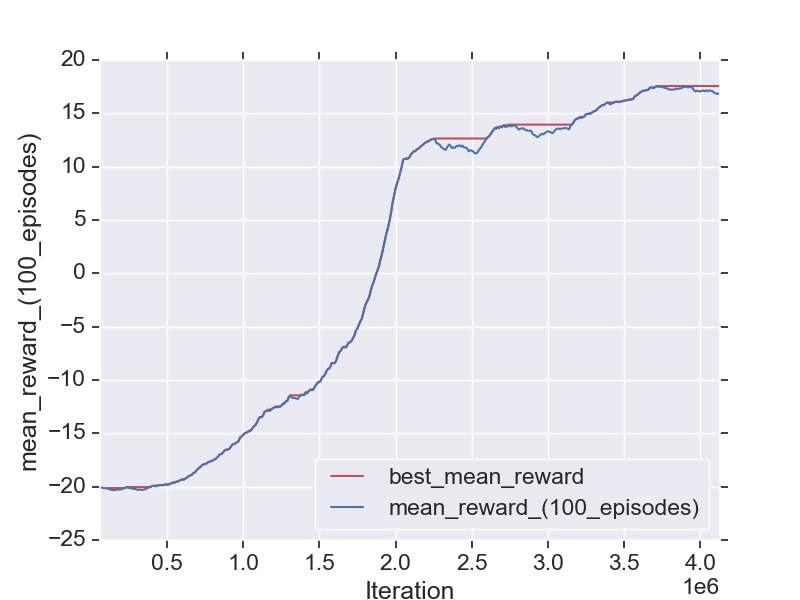
\includegraphics[width=0.6\textwidth]{question1_1.png}}
	\end{figure}
	\subsection{Question 2: double Q-learning.}
	\begin{figure}[!htbp] 
		\floatbox[{\capbeside\thisfloatsetup{capbesideposition={right,center},capbesidewidth=0.4\textwidth}}]{figure}[\FBwidth]
		{\caption[caption]{
				Performance comparison of double Q-learning and vanilla Q-learning Lunar Lander.\\ \hspace{0.4\textwidth}
				My double DQN (\textcolor{orange}{doubleQ}) is slightly better than the vanilla DQN (\textcolor{blue}{DQN}).I did NOT change any default hyperparameters.
			}\label{fig:DDQN}}
		{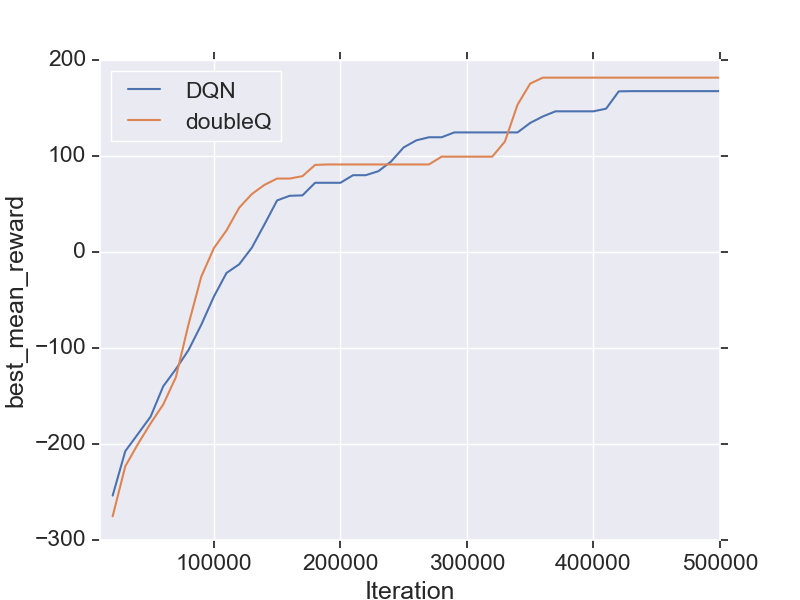
\includegraphics[width=0.6\textwidth]{question1_2.png}}
	\end{figure}
	\pagebreak
	\subsection{Question 3: experimenting with hyperparameters.}
	\begin{figure}[!htbp] 
		\floatbox[{\capbeside\thisfloatsetup{capbesideposition={right,center},capbesidewidth=0.4\textwidth}}]{figure}[\FBwidth]
		{\caption[caption]{
				Hyperparameter tuning of exploration schedule using vanilla DQN on Lunar Lander.\\ 
				\hspace{0.4\textwidth}
				I used the three given Schedule classes in dqn\_utils.py: ConstantSchedule  (\textcolor{orange}{ConstantDQN}), LinearSchedule (\textcolor{green}{LinearDQN}), PiecewiseSchedule (\textcolor{blue}{DQN}).  The default piecewise schedule performs the best in Lunar Lander followed by the linear schedule. Constant schedule performs the worst among all three.
			}\label{fig:hyper}}
		{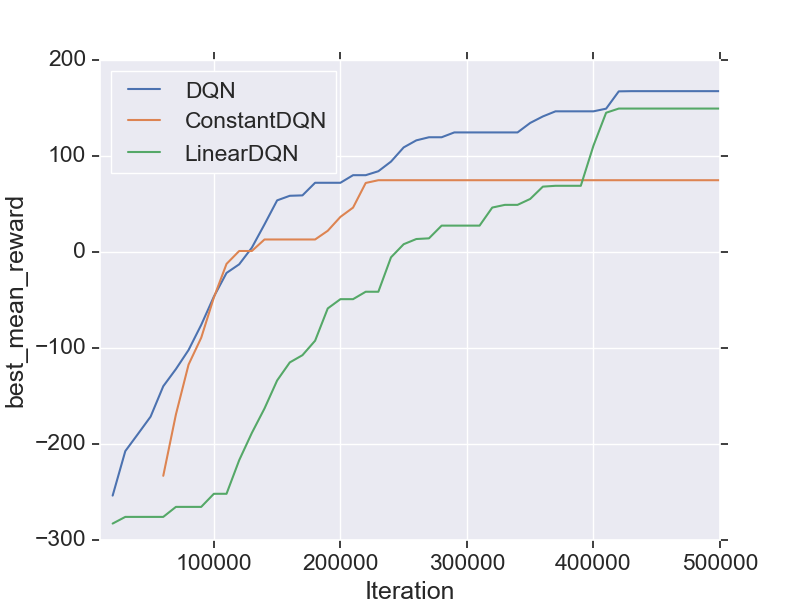
\includegraphics[width=0.6\textwidth]{question1_3.png}}
	\end{figure}
  Constant schedule doesn't do well because exploration at later steps makes the system hard to converge to a stable solution and it always has to consider slightly different new observations.\par
  Piecewise schedule learns faster than the linear schedule might be because the exploration rate decreases so fast in the linear schedule that the system has not picked up enough variety of observations yet.  In an environment with diverse states/observations, it's often good to take a two-step approach: exploring more at the beginning and fitting the collected data later.
  
  \begin{lstlisting}[language=Python]
  # Question 1
  # To run the analysis, use the following line
  python run_dqn_atari.py
  # To plot the result, use the following line
  python multiplot.py data\qlearn_exp_PongNoFrameskip-v4_24-09-2018_10-10-51 --value best_mean_reward mean_reward_(100_episodes) --legend best_mean_reward mean_reward_(100_episodes)
  
  # Question 2
  # To run the analysis, use the following line
  python run_dqn_lander.py
  python run_dqn_lander.py --doubleQ --exp_name doubleQ
  # To plot the result, use the following line
  python plot.py data\qlearn_DQN_LunarLander-v2_25-09-2018_22-47-04 data\qlearn_doubleQ_LunarLander-v2_27-09-2018_18-56-47 --value best_mean_reward
  
  # Question 3
  # To run the analysis, use the following line
  python run_dqn_lander.py
  python run_dqn_lander.py --schedule ConstantSchedule --exp_name ConstantDQN
  python run_dqn_lander.py --schedule LinearSchedule --exp_name LinearDQN
  # To plot the result, use the following line
  python plot.py data\qlearn_DQN_LunarLander-v2_25-09-2018_22-47-04 data\qlearn_ConstantDQN_LunarLander-v2_25-09-2018_23-52-17 data\qlearn_LinearDQN_LunarLander-v2_26-09-2018_00-15-31 --value best_mean_reward
  
  \end{lstlisting}
  
  \pagebreak
   
   

  \section{Actor-Critic}
  \subsection{Question 1: Sanity check with Cartpole}
  \begin{figure}[!htbp] 
  	\floatbox[{\capbeside\thisfloatsetup{capbesideposition={right,center},capbesidewidth=0.4\textwidth}}]{figure}[\FBwidth]
  	{\caption[caption]{
  			Target update and gradient update balancing of Actor-Critic algorithm on CartPole-v0.\\
  			\hspace{0.4\textwidth}
  			I used four different setting as required in the instruction: \\
  			\hspace{0.4\textwidth}
  			1 target update and 1 gradient step per target update (\textcolor{blue}{1\_1}),\\
  			\hspace{0.4\textwidth}
			1 target update and 100 gradient step per target update (\textcolor{orange}{1\_100}), \\
			\hspace{0.4\textwidth}
			10 target update and 10 gradient step per target update (\textcolor{green}{10\_10}),\\
			\hspace{0.4\textwidth}
			100 target update and 1 gradient step per target update (\textcolor{red}{100\_1}).
  		}\label{fig:ac}}
  	{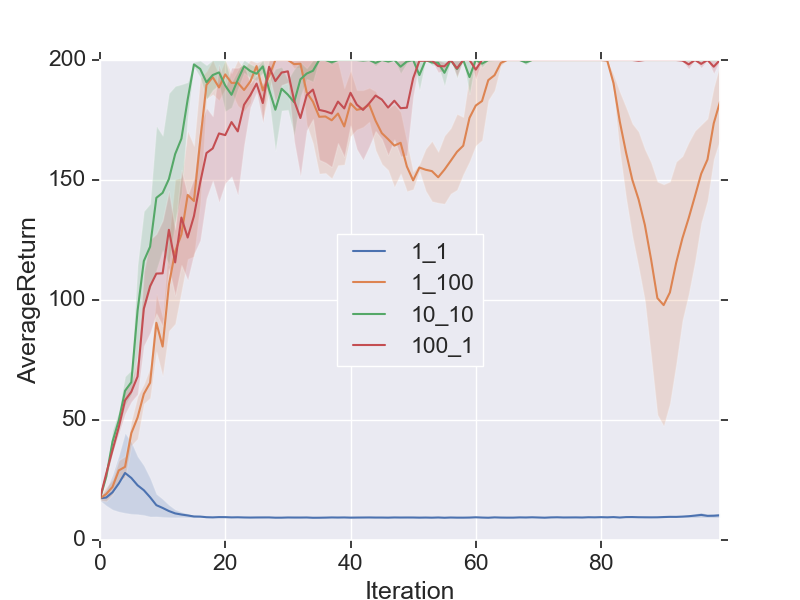
\includegraphics[width=0.6\textwidth]{question2_1.png}}
  \end{figure}
  As we can see, all except \textcolor{blue}{1\_1} reach the maximum reward.  However, \textcolor{orange}{1\_100} is not very stable because running 100 gradient steps per target update might result in a inaccurate target value during gradient update. Once target function is updated, there might be large changes in the reward.  \textcolor{green}{10\_10} gets to the maximum reward faster than \textcolor{red}{100\_1}.  This is simply because policy gets updated more early on due to multiple gradient steps taken.  Only taking one gradient step per update is not enough to have a good performance.  Overall, there is a balance between target update and gradient step per target update.
  
  \pagebreak
  
  \subsection{Question 2: Run actor-critic with more difficult tasks}
  \begin{figure}[!htbp]
  	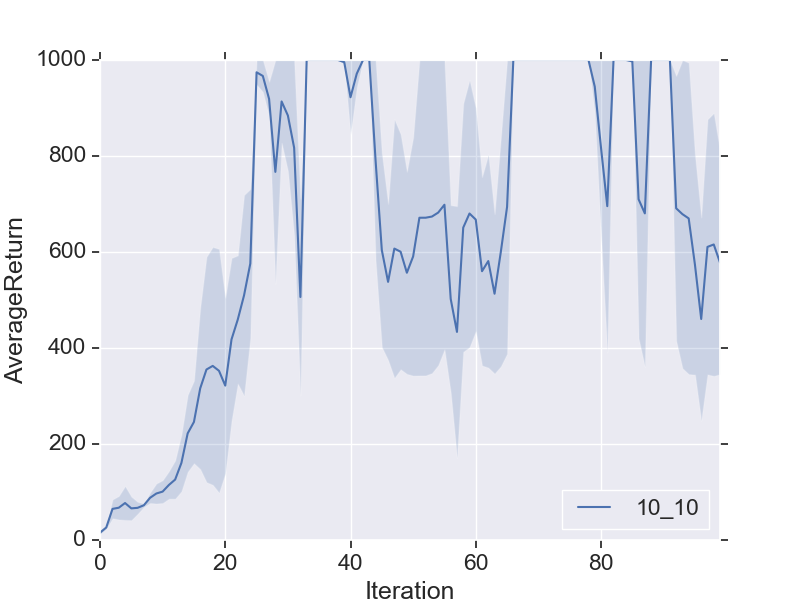
\includegraphics[width=0.48\textwidth]{question2_2a.png}
	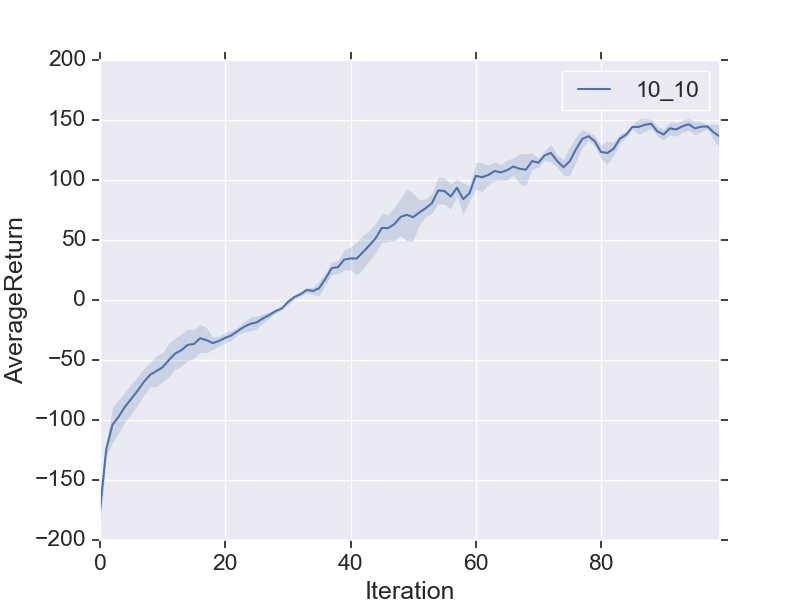
\includegraphics[width=0.48\textwidth]{question2_2b.png}
	\label{fig:ac_diff}
	\caption[caption]{Actor-Critic algorithm on InvertedPendulum (left) and HalfCheetah (right).
	I did NOT change any hyperparameters. Both match the results from policy gradient in HW2.
	}
  \end{figure}
	
  \section{Bonus}
  \begin{figure}[!htbp]
  	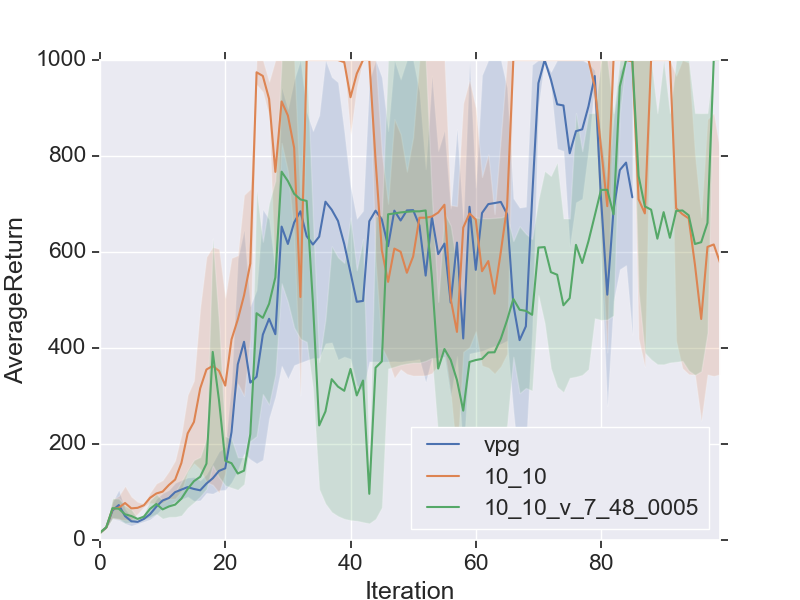
\includegraphics[width=0.48\textwidth]{bonus1.png}
  	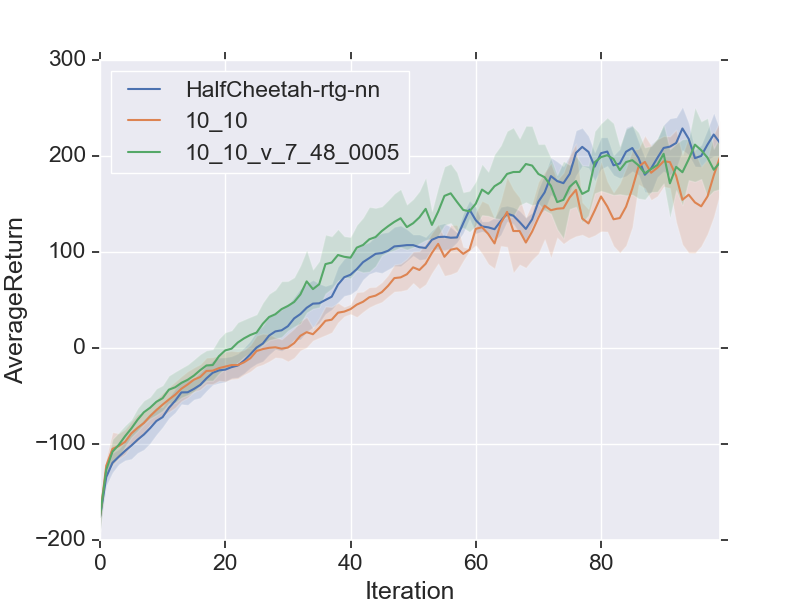
\includegraphics[width=0.48\textwidth]{bonus2.png}
  	\label{fig:bonus}
  	\caption[caption]{Hyperparameter tuning of the critic network on InvertedPendulum (left) and HalfCheetah (right).
  	Left: policy gradient (\textcolor{blue}{vpg}), actor-critic (\textcolor{orange}{10\_10}), actor-critic with independent critic network (\textcolor{green}{10\_10\_v\_7\_48\_0005});
  	Right: policy gradient with normalization (\textcolor{blue}{HalfCheetah-rtg-nn}), actor-critic (\textcolor{orange}{10\_10}), actor-critic with independent critic network (\textcolor{green}{10\_10\_v\_7\_48\_0005}).\\
  	\hspace{0.4\textwidth} 
  	We can see that by implementing an independent critic, the overall performance is indeed improved in both environments.  However, because the original solution is already close to optimal, we don't really see a big improvements by having a more expressive critic network.\\
  	\hspace{0.4\textwidth}
  	The hyperparameters I used for the critic network are as following:\\
  	\hspace{0.4\textwidth}
  	number of hidden layers: $7$, 
  	number of hidden units per layer: $48$, 
  	learning rate: $0.005$.
  	I also changed the discount factor of HalfCheetah to $0.95$.  All other hyperparameters are the same as the default in actor-critic.
  	}
  \end{figure}

  \pagebreak

  \begin{lstlisting}[language=Python]
	## Actor-critic
	# Question 1.
	# To run the analysis, use the following line
	python train_ac_f18.py CartPole-v0 -n 100 -b 1000 -e 3 --exp_name 1_1 -ntu 1 -ngsptu 1
	python train_ac_f18.py CartPole-v0 -n 100 -b 1000 -e 3 --exp_name 100_1 -ntu 100 -ngsptu 1
	python train_ac_f18.py CartPole-v0 -n 100 -b 1000 -e 3 --exp_name 1_100 -ntu 1 -ngsptu 100
	python train_ac_f18.py CartPole-v0 -n 100 -b 1000 -e 3 --exp_name 10_10 -ntu 10 -ngsptu 10
	
	# To plot the result, use the following line
	python plot.py data\ac_1_1_CartPole-v0_27-09-2018_19-36-12 data\ac_1_100_CartPole-v0_27-09-2018_19-42-41 data\ac_10_10_CartPole-v0_27-09-2018_19-45-46 data\ac_100_1_CartPole-v0_27-09-2018_19-39-10
	
	
	# Question 2.
	# To run the analysis, use the following line
	python train_ac_f18.py InvertedPendulum-v2 -ep 1000 --discount 0.95 -n 100 -e 3 -l 2 -s 64 -b 5000 -lr 0.01 --exp_name 10_10 -ntu 10 -ngsptu 10
	python train_ac_f18.py HalfCheetah-v2 -ep 150 --discount 0.95 -n 100 -e 3 -l 2 -s 32 -b 30000 -lr 0.02 --exp_name 10_10 -ntu 10 -ngsptu 10
	
	# To plot the result, use the following line
	python plot.py data\ac_10_10_InvertedPendulum-v2_27-09-2018_19-56-45 ..\hw2\data\vpg_InvertedPendulum-v2_16-09-2018_17-32-43
	python plot.py data\ac_10_10_HalfCheetah-v2_28-09-2018_13-44-24 ..\hw2\data\HalfCheetah-rtg-nn_HalfCheetah-v2_18-09-2018_10-43-21 ..\hw2\data\HalfCheetah_HalfCheetah-v2_17-09-2018_23-52-16
	# ac_10_10_HalfCheetah-v2_27-09-2018_20-09-29
	
	
	# Bonus
	# To run the analysis, use the following line
	python train_ac_f18_bonus.py HalfCheetah-v2 -ep 150 --discount 0.95 -n 100 -e 3 -l 2 -s 32 -b 30000 -lr 0.02 --exp_name 10_10_v_7_48_0005 -ntu 10 -ngsptu 10 -vl 7 -vs 48 -vlr 0.005
	python train_ac_f18_bonus.py InvertedPendulum-v2 -ep 1000 --discount 0.95 -n 100 -e 3 -l 2 -s 64 -b 5000 -lr 0.01 --exp_name 10_10_v_7_48_0005 -ntu 10 -ngsptu 10 -vl 7 -vs 48 -vlr 0.005
	
	# To plot the result, use the following line
	python plot.py ..\hw2\data\HalfCheetah-rtg-nn_HalfCheetah-v2_18-09-2018_10-43-21 data\ac_10_10_HalfCheetah-v2_28-09-2018_13-44-24 data\ac_10_10_v_7_48_0005_HalfCheetah-v2_28-09-2018_22-07-19
	python plot.py ..\hw2\data\vpg_InvertedPendulum-v2_16-09-2018_17-32-43 data\ac_10_10_InvertedPendulum-v2_27-09-2018_19-56-45 data\ac_10_10_v_7_48_0005_InvertedPendulum-v2_29-09-2018_00-15-23
  \end{lstlisting}
	
\end{document}